\chapter{Subordinación y coordinación} \label{ch:subord-coord-es}

\epigraph{If I were a cinnamon peeler\\
I would ride your bed\\
and leave the yellow bark dust\\
on your pillow.}{Michael Ondaatje, \enquote{The Cinnamon Peeler}}

\begin{tblsframedsymbol}{Objetivos de aprendizaje}{bulb}
\begin{itemize}[noitemsep, leftmargin=*]
    \item Distinguir entre subordinación, que crea dependencia jerárquica, y coordinación, que une elementos de igual estatus.
    \item Identificar y analizar oraciones matriz, principales y subordinadas en oraciones complejas.
    \item Reconocer distintos tipos de oraciones subordinadas: de contenido, comparativas y de relativo.
    \item Entender que los subordinadores y los coordinadores funcionan como marcadores estructurales, no como núcleos.
    \item Analizar estructuras coordinadas, incluida la coordinación de sintagmas y de oraciones.
    \item Aplicar pruebas diagnósticas para determinar relaciones estructurales en oraciones complejas.
    \item Reconocer cómo la subordinación y la coordinación colaboran para crear cohesión textual.
    \item Valorar la utilidad pedagógica de estas estructuras para desarrollar conciencia sintáctica.
\end{itemize}
\end{tblsframedsymbol}

\section{Introducción}

La lengua nos permite expresar no solo ideas individuales, sino también relaciones entre ideas. Dos formas fundamentales de hacerlo son la \term{subordinación} (\term{subordination}) y la \term{coordinación} (\term{coordination}). Cada una cumple una función distinta: la subordinación crea jerarquías de dependencia, mientras que la coordinación une elementos de igual estatus.

Considere estas tres formas de conectar las mismas ideas básicas:

\ea \label{ex:intro-es}
    \ea \gll Kim left. Pat came.\\
        Kim irse-PAS Pat venir-PAS\\
    \glt `Kim se fue. Pat vino.' [separadas]
    \ex \gll The fact {\ob}that Kim left{\cb} enabled Pat's arrival.\\
        el hecho Sdr Kim irse-PAS permitir-PAS llegada de-Pat\\
    \glt `El hecho de que Kim se fuera permitió la llegada de Pat.' [subordinada]
    \ex \gll Kim left and Pat came.\\
        Kim irse-PAS y Pat venir-PAS\\
    \glt `Kim se fue y Pat vino.' [coordinada]
    \z
\z
En (\ref{ex:intro-es}a), tenemos dos enunciados independientes. En (b), \mention{that Kim left} está incrustada en una estructura mayor: funciona como complemento dentro del sujeto. En (c), las dos oraciones están puestas al mismo nivel: se presentan como iguales y simplemente están unidas por \mention{and}.

Este contraste entre jerarquía e igualdad atraviesa la gramática. Cuando subordinamos una oración a otra, creamos una relación de dependencia: una oración sirve como complemento o modificador de un elemento de la otra. Cuando coordinamos elementos, afirmamos que tienen igual estatus dentro de la estructura, aunque difieran en otros aspectos.

Las herramientas que usamos para estas relaciones son pocas: palabras como \mention{that} y \mention{whether} para las relaciones de dependencia, y palabras como \mention{and}, \mention{or} y \mention{but} para las relaciones de igualdad. Sin embargo, estas palabras pequeñas nos permiten construir significados complejos a partir de partes simples, mostrar cómo se relacionan las ideas y guiar al lector a través de largas cadenas de razonamiento. Estos elementos señalan una relación gramatical; no funcionan como núcleos.

En este capítulo veremos cómo funcionan estos dos sistemas, por separado y juntos. Veremos cómo la subordinación permite insertar una idea dentro de otra, creando capas de significado. Examinaremos cómo la coordinación permite construir ideas complejas sin perder simplicidad estructural. Y veremos cómo ambos sistemas se complementan y nos dan flexibilidad para expresar casi cualquier relación imaginable entre ideas.

\section{Subordinación}\label{sec:subordination-es}

Cuando nos comunicamos, a menudo necesitamos expresar relaciones complejas entre ideas. A veces una idea depende de otra; a veces un pensamiento sirve para modificar o explicar otro. Aquí entra la subordinación. La \term{subordinación} es el proceso gramatical por el que convertimos una oración en un \term{dependiente} (\term{dependent}) dentro de otra estructura.

Una oración que contiene una \term{oración subordinada} (\term{subordinate clause}) se llama \term{oración matriz} (\term{matrix clause}); una oración que no está contenida en una matriz se llama \term{oración principal} (\term{main clause}). Una oración puede ser al mismo tiempo principal y matriz, como muestra el ejemplo siguiente.

\ea \label{ex:sub-basic-es}
    \ea \gll Kim left early.\\
        Kim irse-PAS temprano\\
    \glt `Kim se fue temprano.' [principal]
    \ex \gll She thinks {[}that Kim left early{]}.\\
        ella pensar-PRES {[}Sdr Kim irse-PAS temprano{]}\\
    \glt `Ella piensa que Kim se fue temprano.' [subordinada]
    \ex \gll {[}She thinks that Kim left early{]}.\\
        {[}ella pensar-PRES Sdr Kim irse-PAS temprano{]}\\
    \glt `Ella piensa que Kim se fue temprano.' [principal/matriz]
    \z
\z
(\ref{ex:sub-basic-es}a) es una oración principal simple. En (b), esa misma oración, entre corchetes en el original, se ha vuelto subordinada; ahora es un dependiente dentro de su oración matriz (c), que también es la oración principal.

Este patrón puede extenderse. En (\ref{ex:sub-basic2-es}), la oración de (\ref{ex:sub-basic-es}b) ha pasado de oración principal a oración subordinada, aunque sigue siendo la matriz de \mention{that Kim left}. En otras palabras, una oración no solo puede ser principal y matriz a la vez; también puede ser subordinada y matriz a la vez.

\ea\label{ex:sub-basic2-es}
\gll I heard {\ob}that she thinks {\ob}that Kim left early{\cb}{\cb}.\\
    yo oír-PAS Sdr ella pensar-PRES Sdr Kim irse-PAS temprano\\
\glt `Oí que ella piensa que Kim se fue temprano.' [subordinada]
\z

Sin embargo, ninguna oración puede ser a la vez una \term{oración principal} y una \term{oración subordinada}. \term{Oración matriz} y \term{oración subordinada} son términos relacionales: expresan la posición de una oración con respecto a otra. \term{Oración principal}, en cambio, refleja un tipo sintáctico cuya estructura no siempre se conserva en los distintos tipos de oraciones subordinadas.

\subsection{Tipos de oraciones subordinadas}

El inglés tiene tres grandes tipos de oraciones subordinadas finitas:\footnote{\textit{CGEL} distingue también entre subordinadas finitas y no finitas, de varios tipos, pero no las trataré aquí.} \term{oraciones de contenido} (\term{content clauses}), \term{oraciones comparativas} (\term{comparative clauses}) y \term{oraciones de relativo} (\term{relative clauses}). Veámoslas por orden:

\ea \label{ex:sub-types-es}
    \ea \gll I doubt that we ordered enough books.\\
        yo dudar-PRES Sdr nosotros pedir-PAS suficientes libros\\
    \glt `Dudo que hayamos pedido suficientes libros.' [contenido]
    \ex \gll More books arrived than we had ordered.\\
        más libros llegar-PAS que nosotros haber-PAS pedido\\
    \glt `Llegaron más libros de los que habíamos pedido.' [comparativa]
    \ex \gll The books that we ordered arrived.\\
        los libros Rel nosotros pedir-PAS llegar-PAS\\
    \glt `Llegaron los libros que habíamos pedido.' [de relativo]
    \z
\z
Las oraciones de contenido son el caso por defecto: no tienen las propiedades sintácticas especiales de las relativas ni de las comparativas. Las oraciones de relativo son el tema del capítulo siguiente, así que aquí consideraremos primero las oraciones de contenido y después las comparativas.

\subsubsection{Oraciones de contenido}

Las oraciones de contenido tienen dos clases principales: declarativas e interrogativas, como en (\ref{ex:content-types-es}).\footnote{\textit{CGEL} también trata las oraciones de contenido exclamativas, pero son bastante raras.}

\ea \label{ex:content-types-es}
    \ea \gll She said that it was genuine.\\
        ella decir-PAS Sdr eso ser-PAS auténtico\\
    \glt `Ella dijo que era auténtico.' [declarativa]
    \ex \gll She asked whether it was genuine.\\
        ella preguntar-PAS si eso ser-PAS auténtico\\
    \glt `Ella preguntó si era auténtico.' [interrogativa básica]
    \ex \gll She asked what made it genuine.\\
        ella preguntar-PAS qué hacer-PAS eso auténtico\\
    \glt `Ella preguntó qué lo hacía auténtico.' [interrogativa focalizada]
    \z
\z
Las palabras \mention{that} y \mention{whether} en (\ref{ex:content-types-es}a y b) hacen un trabajo importante: marcan sus respectivas oraciones como subordinadas. Esto nos lleva a una categoría nueva, importante pero muy pequeña: el \term{subordinador} (\term{subordinator}, Sdr). Los miembros principales de esta categoría son \mention{that} y \mention{whether}, junto con \mention{if} cuando significa `whether', no el \mention{if} condicional. Los subordinadores son especiales porque, a diferencia de otras categorías léxicas, no proyectan sintagmas. Los nombres tienen SN y los verbos tienen SV, pero los subordinadores no tienen SdrP. En cambio, funcionan puramente como marcadores, señalando cómo se relaciona su oración con la estructura mayor. La estructura arbórea se muestra en la figura~\ref{fig:sub-tree-sub-es}. (Los triángulos indican que hay algo de estructura oculta. Véase el capítulo 6.)

\begin{figure}
    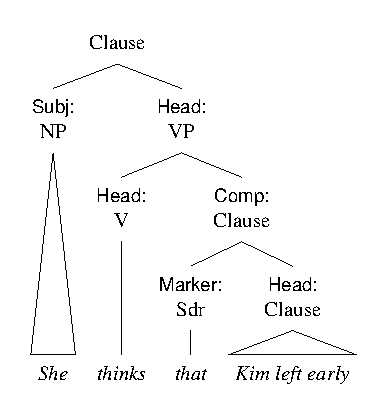
\includegraphics[width=0.55\linewidth]{figures/she thinks that kim left.pdf}
    \caption{Árbol sintáctico que muestra la subordinación: \mention{that Kim left early} como complemento en \mention{She thinks that Kim left early}}\label{fig:sub-tree-sub-es}
\end{figure}

Observe que, en la estructura subordinada, \mention{that} aparece como marcador: no proyecta su propio sintagma, sino que simplemente señala el inicio de la oración subordinada. Un \term{marcador} (\term{marker}, Mk) es un tipo de dependiente que señala cómo se relaciona gramaticalmente su núcleo con la estructura mayor.

Las oraciones de contenido pueden funcionar de varias maneras dentro de la estructura mayor:

\ea \label{ex:content-funcs-es}
    \ea \gll I suspect {\ob}that he left{\cb}.\\
        yo sospechar-PRES Sdr él irse-PAS\\
    \glt `Sospecho que se fue.' [en SV]
    \ex \gll The fact {\ob}that he left{\cb} is clear.\\
        el hecho Sdr él irse-PAS ser-PRES claro\\
    \glt `El hecho de que se fuera es claro.' [en SN]
    \ex \gll I'm glad {\ob}that he left{\cb}.\\
        yo-estar contento Sdr él irse-PAS\\
    \glt `Me alegra que se haya ido.' [en SAdj]
    \ex \gll We can proceed provided {\ob}that he left{\cb}.\\
        nosotros poder-PRES seguir siempre-que Sdr él irse-PAS\\
    \glt `Podemos seguir siempre que se haya ido.' [en SP]
    \ex \gll Whether or not he left is unclear.\\
        si o no él irse-PAS ser-PRES poco-claro\\
    \glt `No está claro si se fue o no.' [sujeto]
    \ex \gll It's unclear whether or not he left.\\
        ello-estar poco-claro si o no él irse-PAS\\
    \glt `No está claro si se fue o no.' [sujeto extrapuesto]
    \z
\z

En las oraciones de contenido declarativas, el marcador, es decir, el subordinador \mention{that}, puede ser obligatorio, opcional o inadmisible según la función de la oración:
\ea\label{ex:marker-need-es}
    \ea \gll That Kim left surprised no one.\\
        Sdr Kim irse-PAS sorprender-PAS nadie\\
    \glt `Que Kim se fuera no sorprendió a nadie.' [obligatorio]
    \ex \gll I know that Kim left.\\
        yo saber-PRES Sdr Kim irse-PAS\\
    \glt `Sé que Kim se fue.' [opcional]
    \ex \gll *We left before that Kim arrived.\\
        *nosotros irse-PAS antes Sdr Kim llegar-PAS\\
    \glt `Sentido previsto: nos fuimos antes de que llegara Kim. En inglés, \mention{that} no puede aparecer aquí.' [*; inadmisible]
\z
\z
Las oraciones sujeto como (\ref{ex:marker-need-es}a) siempre necesitan un marcador. Como complementos, las declarativas pueden aparecer casi siempre con o sin marcador, como en (b). La principal excepción se da cuando funcionan como complementos dentro de SP, como en (c).

\label{sec:sub-interrog-es}

Las oraciones de contenido interrogativas son interesantes porque difieren sintácticamente de las interrogativas de oración principal. Mientras que las interrogativas básicas de oración principal pueden identificarse por la inversión sujeto--auxiliar (\mention{Did she accept?}), sus equivalentes subordinadas marcan su naturaleza interrogativa con \mention{whether} o \mention{if}:

\ea interrogativas básicas\label{ex:int-sub-es}
    \ea \gll Did she accept?\\
        AUX ella aceptar\\
    \glt `¿Aceptó?' [principal, invertida]
    \ex \gll I wonder {\ob}whether she accepted{\cb}.\\
        yo preguntarse-PRES si ella aceptar-PAS\\
    \glt `Me pregunto si aceptó.' [subordinada]
    \z
\z
\ea interrogativas focalizadas
    \ea \gll How did we get here?\\
        cómo AUX nosotros llegar aquí\\
    \glt `¿Cómo llegamos aquí?' [principal, invertida]
    \ex \gll I wonder {\ob}how we got here{\cb}.\\
        yo preguntarse-PRES cómo nosotros llegar-PAS aquí\\
    \glt `Me pregunto cómo llegamos aquí.' [subordinada]
    \z
\z
Esto es difícil para quienes aprenden inglés. Los principiantes normalmente no invierten nada y forman mal las interrogativas principales. Los estudiantes con más experiencia, al haber comprendido la inversión, la aplican en todas partes y estructuran mal las interrogativas subordinadas. Solo en niveles bastante altos los estudiantes distinguen cómodamente las dos posibilidades.

Esta diferencia estructural entre interrogativas principales y subordinadas, sin embargo, empieza a debilitarse a medida que la inversión continúa su lenta expansión. Aunque todavía es raro ver oraciones de contenido interrogativas invertidas en la escritura, ejemplos como (\ref{ex:non-inverted-interrogative-es}) se han vuelto bastante comunes en el habla. En unos siglos, la inversión quizá sea la norma para todas las interrogativas y los marcadores quizá se vuelvan opcionales. Yo no me quedaría esperando.

\ea\label{ex:non-inverted-interrogative-es}
\gll We need a story of {\ob}how did we get here{\cb}.\\
    nosotros necesitar-PRES una historia de cómo AUX nosotros llegar aquí\\
\glt `Necesitamos una historia de cómo llegamos aquí.'
\z
Por ahora, sin embargo, un marcador, normalmente \mention{whether} o \mention{if}, sigue siendo obligatorio en las oraciones de contenido interrogativas básicas. De lo contrario, sería imposible distinguirlas de las declarativas no marcadas en la mayoría de los casos.

\subsubsection*{El mandativo}

Un subtipo especial de construcción subordinada es el \term{mandativo} (\term{mandative}), que aparece con predicados que expresan requisito o necesidad:

\ea \label{ex:mandative-es}
    \ea \gll It is essential {\ob}that he be there{\cb}.\\
        ello ser-PRES esencial Sdr él estar-FORMA.SIMPLE allí\\
    \glt `Es esencial que esté allí.' [subjuntivo]
    \ex \gll It is essential {\ob}that he should be there{\cb}.\\
        ello ser-PRES esencial Sdr él should estar allí\\
    \glt `Es esencial que esté allí.' [should]
    \ex \gll It is essential {\ob}that he is there{\cb}.\\
        ello ser-PRES esencial Sdr él estar-PRES allí\\
    \glt `Es esencial que está allí.' [indicativo]
    \z
\z
La variante de \term{subjuntivo} (\term{subjunctive}) usa la forma simple del verbo, mientras que la variante con \mention{should} es, o al menos solía ser, más común en el inglés británico. El inglés americano tiende a preferir el subjuntivo. La variante de \term{indicativo} (\term{indicative}) usa una forma ordinaria con tiempo.

Este es un buen ejemplo de cómo las variaciones en las subordinadas pueden llevar diferencias sutiles de significado y mostrar preferencias regionales. Para fines de enseñanza, vale la pena notar que la forma indicativa se está haciendo más común, especialmente en contextos informales, aunque el subjuntivo sigue siendo estándar en la escritura formal.

\begin{tblsframedsymbol}{Compruebe su comprensión: matriz y subordinada}{test}
Practique la identificación de relaciones estructurales:
\begin{itemize}[noitemsep, leftmargin=*]
    \item En \mention{I know that she thinks that he left}, identifique la oración principal, las oraciones matriz y las subordinadas.
    \item Explique por qué \mention{She asked whether he left} no tiene inversión pero \mention{Did he leave?} sí.
    \item Encuentre la estructura mandativa: \mention{It's important that he be careful} frente a \mention{It's important that he is careful}.
\end{itemize}
Comprender estas relaciones estructurales ayuda a aclarar cómo surge el significado de la arquitectura sintáctica.
\end{tblsframedsymbol}

\subsection{Oraciones comparativas}

El segundo gran tipo de subordinada finita es la oración comparativa. Estas oraciones completan una comparación, como en (\ref{ex:comparative-intro-es}).

\ea \label{ex:comparative-intro-es}
    \ea \gll The ice was thicker than {\ob}we expected{\cb}.\\
        el hielo ser-PAS más-grueso que nosotros esperar-PAS\\
    \glt `El hielo era más grueso de lo que esperábamos.'
    \ex \gll She writes faster than {\ob}she speaks{\cb}.\\
        ella escribir-PRES más-rápido que ella hablar-PRES\\
    \glt `Escribe más rápido de lo que habla.'
    \ex \gll It doesn't cost as much as {\ob}I'd thought{\cb}.\\
        ello NEG costar-PRES tanto como yo-haber-PAS pensar\\
    \glt `No cuesta tanto como había pensado.'
    \z
\z
Lo que distingue a las comparativas de las oraciones de contenido es que incluyen elipsis: dejan fuera elementos que pueden recuperarse del contexto. En (\ref{ex:comparative-ellipsis-es}), los puntos suspensivos indican la elipsis.\footnote{En un capítulo anterior introduje los huecos. Los huecos difieren de la elipsis porque son elementos estructurales en los árboles; la elipsis es material recuperable semánticamente a partir del contexto, pero no un elemento sintáctico.}

\ea \label{ex:comparative-ellipsis-es}
    \ea \gll Kim read more books than {\ob}Pat read \dots{\cb}.\\
        Kim leer-PAS más libros que Pat leer-PAS \dots\\
    \glt `Kim leyó más libros de los que leyó Pat.'
    \ex \gll Kim read more books than {\ob}Pat did \dots{\cb}.\\
        Kim leer-PAS más libros que Pat AUX.PAS \dots\\
    \glt `Kim leyó más libros que Pat.'
    \ex \gll Kim read more books than {\ob}Pat{\cb}.\\
        Kim leer-PAS más libros que Pat\\
    \glt `Kim leyó más libros que Pat.'
    \z
\z

Las dos primeras variantes muestran elipsis; en (b), la proforma \mention{did} aparece en lugar de repetir \mention{read}. La tercera, (c), tiene \mention{Pat} como complemento de SN, no como complemento oracional. Las tres significan básicamente lo mismo.

A diferencia de la mayoría de los casos de elipsis, en las comparativas es agramatical proporcionar la información omitida: *\mention{Kim read more books than Pat read 20 books} o *\mention{It's not as deep as it is 20 cm wide}. La elipsis es parte esencial de este tipo de oración. La estructura de la comparativa se muestra en la figura~\ref{fig:comp-tree-es}.

\begin{figure}
    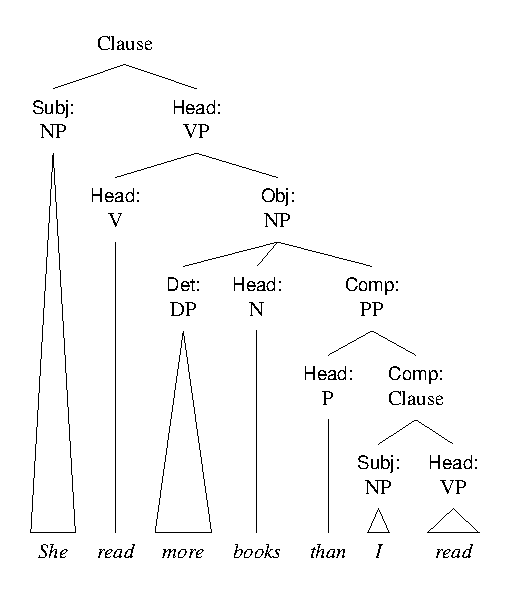
\includegraphics[width=0.7\linewidth]{figures/she read more books than I read.pdf}
    \caption{Árbol sintáctico que muestra una oración comparativa con elipsis}\label{fig:comp-tree-es}
\end{figure}

Las comparativas funcionan como complementos dentro de un SP con \mention{than} o \mention{as}, según el tipo de comparación que se haga.

\ea \label{ex:comp-markers-es}
    \ea \gll Kim is taller than {\ob}Pat is{\cb}.\\
        Kim ser-PRES más-alto que Pat ser-PRES\\
    \glt `Kim es más alta que Pat.' [desigualdad]
    \ex \gll Kim is as tall as {\ob}Pat is{\cb}.\\
        Kim ser-PRES tan alta como Pat ser-PRES\\
    \glt `Kim es tan alta como Pat.' [igualdad\footnote{El término \emph{igualdad} puede ser algo engañoso aquí. El ejemplo significa que Kim es al menos tan alta como Pat; incluso puede ser más alta.}]
    \z
\z
\mention{Than} en (\ref{ex:comp-markers-es}a) indica desigualdad, mientras que \mention{as} en (b) marca igualdad. El primer \mention{as} es un adverbio: tenemos el SAdj \mention{as tall}, con \mention{as} como modificador. El segundo es una preposición.

Para quienes aprenden inglés, las comparativas presentan varios retos:
\begin{itemize}[noitemsep]
    \item entender cuándo y cuánto material puede elidirse;
    \item dominar los distintos patrones de igualdad y desigualdad;
    \item manejar comparaciones complejas con varios elementos.
\end{itemize}

La buena noticia es que las comparativas siguen patrones bastante regulares. Los aprendices suelen dominar las formas básicas, como \mention{taller than} `más alto que' y \mention{as tall as} `al menos tan alto como', antes de enfrentarse a estructuras más complejas.

\section{Coordinación}\label{sec:coordination-es}

Mientras que la subordinación crea relaciones de dependencia entre oraciones, la \term{coordinación} une elementos de igual estatus sintáctico. En el centro de este sistema hay una pequeña clase cerrada de palabras llamadas \term{coordinadores} (\term{coordinators}, Crd), principalmente \mention{and}, \mention{or} y \mention{but} (se necesitan los tres incluso para enumerarlos). Igual que los subordinadores, los coordinadores funcionan como marcadores.

Una advertencia sobre \term{coordinación}: aquí no significa simplemente que dos ideas estén conectadas de manera coherente en el discurso. Es una relación estructural precisa. Los elementos coordinados tienen el mismo estatus sintáctico, y ninguno funciona como núcleo del conjunto.

Considere estos ejemplos:

\ea \label{ex:coord-basic-es}
    \ea \gll {\ob}Jane is a good teacher{\cb} {\ob}and her students really like her{\cb}.\\
        Jane ser-PRES una buena profesora y sus estudiantes realmente querer-PRES ella\\
    \glt `Jane es una buena profesora y sus estudiantes la quieren mucho.'
    \ex \gll They offered us a choice of {\ob}red wine{\cb}, {\ob}white wine{\cb}, {\ob}or beer{\cb}.\\
        ellos ofrecer-PAS nos una opción de rojo vino blanco vino o cerveza\\
    \glt `Nos ofrecieron elegir entre vino tinto, vino blanco o cerveza.'
    \ex \gll Her assistant is {\ob}very young{\cb} {\ob}but a quick learner{\cb}.\\
        su asistente ser-PRES muy joven pero una rápida aprendiz\\
    \glt `Su asistente es muy joven pero aprende rápido.'
    \z
\z
Los elementos entre corchetes en estos ejemplos funcionan como \term{coordinados} (\term{coordinates}). Esta función puede realizarse mediante oraciones, como en (\ref{ex:coord-basic-es}a), mediante SN u otros sintagmas, como en (b), o, con menos frecuencia, mediante una mezcla de categorías como el SAdj y el SN en (c). Los coordinadores suelen expresar relaciones distintas: \mention{and} para adición, \mention{or} para alternativas y \mention{but} para contraste.

Lo que diferencia a la coordinación de las construcciones vistas antes es que no tiene núcleo: ningún coordinado es el núcleo de toda la construcción. Esta falta de núcleo se ve en una prueba simple. En la mayoría de los casos, se puede reemplazar toda la coordinación por cualquiera de sus coordinados:

\ea \label{ex:coord-replace-es}
    \ea \gll Her assistant is very young.\\
        su asistente ser-PRES muy joven\\
    \glt `Su asistente es muy joven.'
    \ex \gll Her assistant is a quick learner.\\
        su asistente ser-PRES una rápida aprendiz\\
    \glt `Su asistente aprende rápido.'
    \z
\z
Tanto (\ref{ex:coord-replace-es}a) como (b) son alternativas gramaticales a (\ref{ex:coord-basic-es}c). Esto es muy distinto de las construcciones con núcleo, como \mention{very young}, donde se puede usar solo el núcleo (\mention{she's young}), pero no solo el dependiente (*\mention{she's very}). La estructura de coordinación se muestra en la figura~\ref{fig:coord-basic-es}.

\begin{figure}
    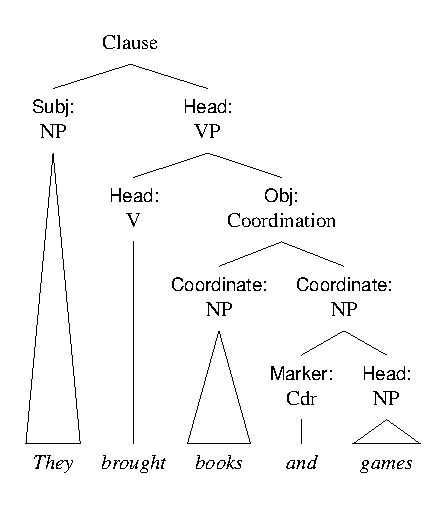
\includegraphics[width=0.65\linewidth]{figures/the brought books and games.pdf}
    \caption{Coordinación básica con marcador: \mention{They brought books and games}}\label{fig:coord-basic-es}
\end{figure}

\subsection{Propiedades de la coordinación}

Tres propiedades principales distinguen la coordinación de otras construcciones.

No hay límite gramatical para el número de coordinados, salvo con \mention{but}:

\ea \label{ex:coord-multiple-es}
\gll Nothing noble, sublime, profound, delicate, tasteful or even decent can find a place.\\
    nada noble sublime profundo delicado de-buen-gusto o incluso decente poder-PRES encontrar un lugar\\
\glt `Nada noble, sublime, profundo, delicado, de buen gusto o siquiera decente puede encontrar lugar.'
\z

Los coordinados deben ser funcionalmente semejantes: deben poder cumplir la misma función si se usan solos.

\ea \label{ex:coordinate-function-es}
    \ea \gll I'll be back next week or at the end of the month.\\
        yo-FUT estar de-vuelta próxima semana o a el final de el mes\\
    \glt `Volveré la semana que viene o a final de mes.' [adjuntos temporales]
    \ex \gll *We're leaving Rome and next week.\\
        *nosotros salir-PRES Roma y próxima semana\\
    \glt `La estructura prevista es incorrecta en inglés: \mention{Rome} es objeto, pero \mention{next week} es adjunto.' [*; objeto y adjunto]
    \z
\z

Un coordinado expandido, es decir, uno que incluye su coordinador, nunca puede moverse al frente:

\ea \label{ex:coord-front-es}
    \ea \gll They attended but they aren't members.\\
        ellos asistir-PAS pero ellos NEG-ser-PRES miembros\\
    \glt `Asistieron, pero no son miembros.'
    \ex \gll *But they aren't members, they attended.\\
        *pero ellos NEG-ser-PRES miembros ellos asistir-PAS\\
    \glt `Sentido previsto: asistieron, pero no son miembros. En inglés, el coordinado expandido con \mention{but} no puede anteponerse así.' [*]
    \z
\z

\subsection{Nota sobre coordinadores al inicio de oración}

Una regla prescriptiva advierte contra comenzar oraciones con coordinadores como \mention{and} o \mention{but}. Esta prohibición no tiene fundamento en la gramática ni en el uso del inglés. Los coordinadores iniciales han sido usados por escritores hábiles a lo largo de la historia del inglés, incluido este libro; encontrará numerosos ejemplos en este capítulo y en otros. Sin embargo, un coordinador al inicio de oración no puede unir su oración con la anterior en una coordinación estrecha: recuerde la restricción de anteposición en (\ref{ex:coord-front-es}). Puede funcionar, en cambio, como \term{conector discursivo} (\term{discourse connector}), señalando cómo se relaciona la nueva oración con lo anterior.

Esta distinción también importa en español: un conector discursivo relaciona tramos del texto, mientras que una coordinación sintáctica relaciona elementos dentro de una misma estructura. La única restricción genuina es estilística: como cualquier recurso, los coordinadores iniciales pueden volverse monótonos si se abusa de ellos. Usados con cuidado, son útiles para manejar el flujo del discurso y señalar relaciones textuales.

\subsection{Tipos de coordinación}

La distinción más simple es entre \term{coordinación simétrica} (\term{symmetric coordination}), donde el orden de los coordinados no importa, y \term{coordinación asimétrica} (\term{asymmetric coordination}), donde sí importa:

\ea \label{ex:coord-sym-es}
    \ea \gll I was hungry and tired.\\
        yo estar-PAS hambriento y cansado\\
    \glt `Tenía hambre y estaba cansado.' [simétrica]
    \ex \gll I got up and had breakfast.\\
        yo levantarse-PAS y tomar-PAS desayuno\\
    \glt `Me levanté y desayuné.' [asimétrica]
    \z
\z
En (\ref{ex:coord-sym-es}a), invertir los coordinados no cambia el significado. Pero en (b), el orden implica secuencia: levantarse ocurrió antes de desayunar.

También distinguimos entre \term{coordinación distributiva} (\term{distributive coordination}) y \term{coordinación conjunta} (\term{joint coordination}):

\ea \label{ex:coord-dist-es}
    \ea \gll Kim and Pat are fine players.\\
        Kim y Pat ser-PRES buenos jugadores\\
    \glt `Kim y Pat son buenos jugadores.' [distributiva]
    \ex \gll Kim and Pat are a good pair.\\
        Kim y Pat ser-PRES una buena pareja\\
    \glt `Kim y Pat forman una buena pareja.' [conjunta]
    \z
\z
En (\ref{ex:coord-dist-es}a), la propiedad de ser buen jugador se aplica a Kim y a Pat individualmente. Pero en (b), formar una buena pareja solo puede aplicarse a los dos juntos; ninguno de los dos podría ser una pareja por sí solo.

\subsection{Marcación de la coordinación}

La coordinación puede marcarse de varias maneras:
\begin{itemize}[noitemsep]
    \item Con un coordinador: \mention{red and blue}
    \item Sin ningún marcador: \mention{red, white, blue}
    \item Con coordinadores repetidos: \mention{red or white or blue}
    \item Con marcadores correlativos: \mention{both red and blue}
\end{itemize}

Aunque los coordinadores suelen expresar adición (\mention{and}), alternativas (\mention{or}) y contraste (\mention{but}), pueden llevar significados adicionales en la coordinación asimétrica:

\ea \label{ex:coord-meaning-es}
    \ea \gll Pay within a week and you'll get a discount.\\
        pagar dentro-de una semana y tú-FUT obtener un descuento\\
    \glt `Paga dentro de una semana y obtendrás un descuento.' [condicional]
    \ex \gll Pay within a week or you'll lose the discount.\\
        pagar dentro-de una semana o tú-FUT perder el descuento\\
    \glt `Paga dentro de una semana o perderás el descuento.' [condicional negativa]
    \z
\z

\begin{tblsframedsymbol}{Reconocimiento de patrones: coordinación o subordinación}{test}
Aplique los diagnósticos para distinguir estas estructuras:
\begin{itemize}[noitemsep, leftmargin=*]
    \item \mention{She thinks that he left} frente a \mention{She left and he stayed}: ¿cuál inserta una oración dentro de otra y cuál une dos oraciones de igual estatus?
    \item \mention{Although it rained, we went} frente a \mention{It rained but we went}: ¿cuál muestra jerarquía de dependencia y cuál muestra igual estatus?
    \item \mention{*But we went, it rained} frente a \mention{Although it rained, we went}: ¿qué revela la anteposición sobre la estructura?
\end{itemize}
Estas pruebas ayudan a distinguir el encajamiento jerárquico de la unión entre elementos de igual estatus.
\end{tblsframedsymbol}

Con la introducción de los coordinadores, ya hemos encontrado todas las categorías léxicas principales del inglés, excepto las interjecciones, así como las principales funciones sintácticas que cumplen en las oraciones.

\subsection{La estructura de la coordinación}

Cuando coordinamos elementos, deben compartir la misma función sintáctica. Esto significa que se pueden coordinar complementos con complementos o modificadores con modificadores, pero no un complemento con un modificador. Compare:

\ea \label{ex:coord-function-es}
    \ea \gll We listened {\ob}to the teacher{\cb} {\ob}and the students{\cb}.\\
        nosotros escuchar-PAS a el profesor y los estudiantes\\
    \glt `Escuchamos al profesor y a los estudiantes.' [complementos]
    \ex \gll We listened {\ob}Monday{\cb} and {\ob}Tuesday{\cb}.\\
        nosotros escuchar-PAS lunes y martes\\
    \glt `Escuchamos el lunes y el martes.' [modificadores]
    \ex \gll *We listened {\ob}to the teachers{\cb} and {\ob}Monday{\cb}.\\
        *nosotros escuchar-PAS a los profesores y lunes\\
    \glt `La estructura prevista es incorrecta en inglés: \mention{to the teachers} es complemento, pero \mention{Monday} es modificador.' [*; funciones mixtas]
    \z
\z
Los elementos coordinados, llamados \term{coordinados}, pueden provenir de cualquier gran tipo de sintagma: nombres, verbos, adjetivos, preposiciones, sintagmas mayores u oraciones. Lo que importa es que funcionen de la misma manera dentro de la estructura mayor.

\subsection{Coordinación con y sin marcadores}

La coordinación puede aparecer con o sin un coordinador explícito. Cuando no hay coordinador, hablamos de \term{coordinación asindética} (\term{asyndetic coordination}):

\ea \label{ex:coord-marking-es}
    \ea \gll She brought {\ob}games{\cb}, {\ob}stories{\cb}, {\ob}songs{\cb}.\\
        ella traer-PAS juegos cuentos canciones\\
    \glt `Trajo juegos, cuentos, canciones.' [asindética]
    \ex \gll She brought {\ob}games{\cb}, {\ob}stories{\cb}, and {\ob}songs{\cb}.\\
        ella traer-PAS juegos cuentos y canciones\\
    \glt `Trajo juegos, cuentos y canciones.' [sindética]
    \z
\z
Además de la coordinación simple con un solo coordinador, podemos tener \term{coordinación correlativa} (\term{correlative coordination}), donde aparecen marcadores con varios coordinados:

\ea \label{ex:coord-correlative-es}
    \ea \gll {\ob}Both{\cb} tired {\ob}and{\cb} hungry\\
        tanto cansado como hambriento\\
    \glt `Tanto cansado como hambriento'
    \ex \gll {\ob}Either{\cb} now {\ob}or{\cb} never\\
        o ahora o nunca\\
    \glt `O ahora o nunca'
    \ex \gll {\ob}Neither{\cb} simple {\ob}nor{\cb} easy\\
        ni simple ni fácil\\
    \glt `Ni simple ni fácil'
    \z
\z

\subsection{Coordinación por niveles}

A veces los coordinados contienen a su vez coordinación, creando lo que llamamos coordinación por niveles. Considere este ejemplo:

\ea \label{ex:coord-layered-es}
\gll The story was {\ob}short and sweet{\cb} but {\ob}complex and thought-provoking{\cb}.\\
    la historia ser-PAS corta y dulce pero compleja y provocadora-de-pensamiento\\
\glt `La historia era breve y encantadora, pero compleja y estimulante.'
\z
Aquí tenemos dos coordinados principales unidos por \mention{but}, pero cada uno contiene su propia coordinación interna con \mention{and}. Esta estratificación permite expresar relaciones complejas entre ideas manteniendo una estructura clara. La estructura por niveles se muestra en la figura~\ref{fig:coord-layered-es}.

\begin{figure}
    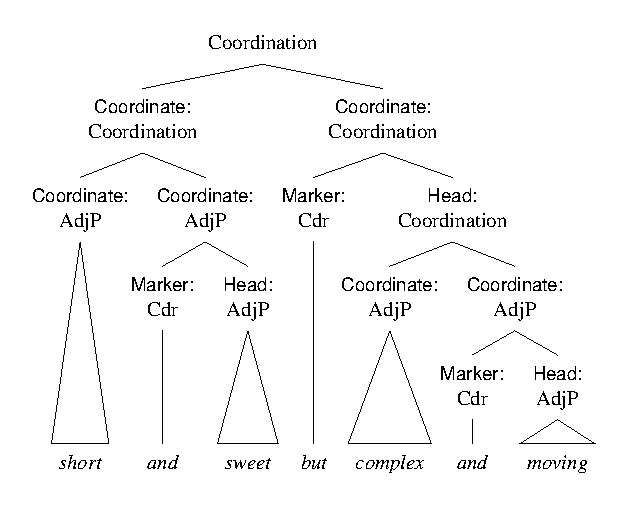
\includegraphics[width=0.9\linewidth]{figures/short and sweet but complex and moving.pdf}
    \caption{Coordinación por niveles: \mention{short and sweet but complex and moving}}\label{fig:coord-layered-es}
\end{figure}

\subsection{Tipos especiales de coordinación}

Un tipo especialmente interesante de coordinación aparece en estructuras comparativas:

\ea \label{ex:coord-comp-es}
    \ea \gll He's as tall as {\ob}or taller than{\cb} his brother.\\
        él-ser tan alto como o más-alto que su hermano\\
    \glt `Es tan alto como su hermano o más alto que él.'
    \ex \gll She writes more {\ob}but understands less{\cb} than before.\\
        ella escribir-PRES más pero entender-PRES menos que antes\\
    \glt `Escribe más pero entiende menos que antes.'
    \z
\z
Estas estructuras suelen incluir relaciones complejas entre los coordinados y los elementos que comparten. Su interpretación requiere entender tanto la coordinación como la relación comparativa.

\begin{tblsframedsymbol}{Autoevaluación rápida: estructuras complejas}{test}
Ponga a prueba su capacidad de analizar estructuras por niveles:
\begin{itemize}[noitemsep, leftmargin=*]
    \item En \mention{I know that she left and he stayed}, identifique todas las relaciones de subordinación y coordinación.
    \item En \mention{Both young and talented, she succeeded}, identifique los marcadores correlativos y los adjetivos coordinados.
    \item Analice la estructura: \mention{He's taller than I thought but shorter than his brother}.
\end{itemize}
Comprender estos patrones complejos ayuda a ver cómo la subordinación y la coordinación trabajan juntas para construir significado.
\end{tblsframedsymbol}

\section{Resumen}

La subordinación y la coordinación hacen el mismo trabajo, conectar ideas, pero con arquitecturas opuestas. La subordinación incrusta; la coordinación une. La buena escritura equilibra ambas. Una vez que se puede reconocer qué estructura intenta construir un estudiante y dónde se rompe, se puede nombrar el problema: demasiadas capas, demasiada enumeración, o un subordinador donde bastaría un coordinador, en lugar de simplemente sentir que algo no encaja.
